\documentclass[review,preprint,12pt]{elsarticle}
%\biboptions{numbers,super,comma}
\biboptions{round,authoryear,semicolon}
\renewcommand{\cite}{\citep} % make default citations parenthetical

\setcounter{secnumdepth}{0}

\usepackage{titlesec}
\titleformat*{\section}{\Large\bfseries}
\titleformat*{\subsection}{\large\bfseries}
\titleformat*{\subsubsection}{\normalsize\itshape}

\usepackage{amsmath}
\usepackage{amssymb}
\usepackage{amsthm}

\usepackage{graphicx}
%\usepackage{natbib}
\usepackage[labelfont=bf]{caption}
\usepackage{subcaption}
\usepackage{hyperref}
% Turn off hyperlinking in list of tables and figures
\makeatletter
\let\Hy@linktoc\Hy@linktoc@none
\makeatother

\usepackage{color}
\usepackage{soul}

\usepackage{diagbox}

\usepackage[nomarkers,tablesfirst,]{endfloat}
%\captionsetup[figure]{labelsep=none,textformat=empty}
\usepackage{floatpag}
\floatpagestyle{empty}
% Rename List of Figures and Tables
\renewcommand\listfigurename{Supplemental Figures}
\renewcommand\listtablename{Table Captions}
% Remove page numbers from List of Figures
\usepackage{tocloft}
\cftpagenumbersoff{figure}
\cftpagenumbersoff{table}
% Make List of Figures have better spacing
\setlength\cftparskip{1em}

\usepackage{fancyhdr}
\pagestyle{fancy}
\fancyhf{}
\renewcommand{\headrulewidth}{0pt}

\rfoot{\center S\thepage}

%\biboptions{numbers,super,comma}

\newtheorem{theorem}{Theorem}
\newtheorem{lemma}[theorem]{Lemma}

\theoremstyle{definition}
\newtheorem{definition}[theorem]{Definition}
\newtheorem{example}[theorem]{Example}
\newtheorem{xca}[theorem]{Exercise}

\theoremstyle{remark}
\newtheorem{remark}[theorem]{Remark}

\renewcommand{\refname}{\normalfont\selectfont\Large \textbf{Supplemental References}} 

%\numberwithin{equation}

%    Absolute value notation
%\newcommand{\abs}[1]{\lvert#1\rvert}

%    Blank box placeholder for figures (to avoid requiring any
%    particular graphics capabilities for printing this document).
\newcommand{\blankbox}[2]{%
  \parbox{\columnwidth}{\centering
%    Set fboxsep to 0 so that the actual size of the box will match the
%    given measurements more closely.
    \setlength{\fboxsep}{0pt}%
    \fbox{\raisebox{0pt}[#2]{\hspace{#1}}}%
  }%
}

\journal{Cell Systems}

\begin{document}

\renewcommand\thefigure{S\arabic{figure}}
\setcounter{figure}{0}
\renewcommand\thetable{S\arabic{table}}
\setcounter{table}{0}

%\section{Supplemental Figures}

\begin{figure}[hbp]
    \centering
    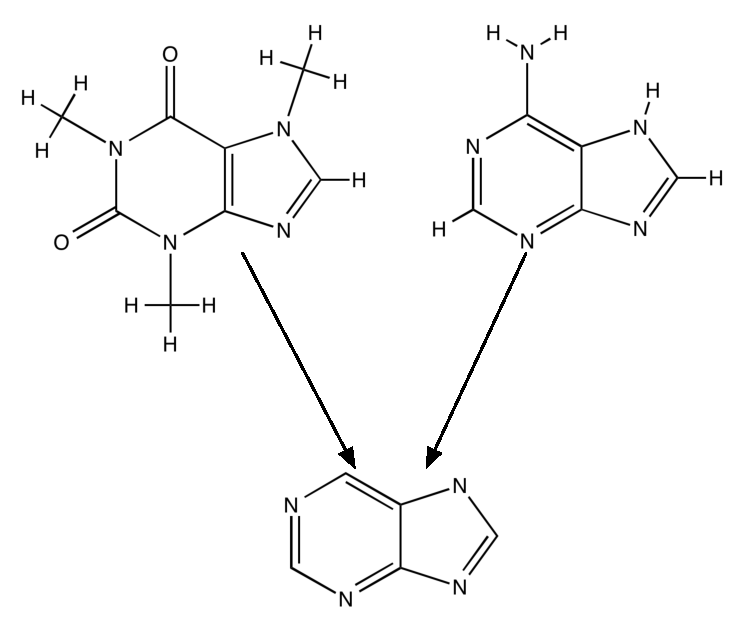
\includegraphics[width=1\textwidth]{assets/ammolite-simplification.pdf}
    \caption{ Ammolite's preprocessing during the clustering phase. Ammolite 
    removes nodes and edges that do not participate in simple cycles, and 
    treats all edges as simple, unlabeled edges. In this example, both caffeine 
    and adenine become a purine-like graph structure. Note that the resulting 
    graph has no implicit hydrogens.
    }
    \label{fig:ammolite}
\end{figure}

\begin{figure}[hbp]
    \centering
    \centerline{
    \begin{subfigure}[b]{4in}
        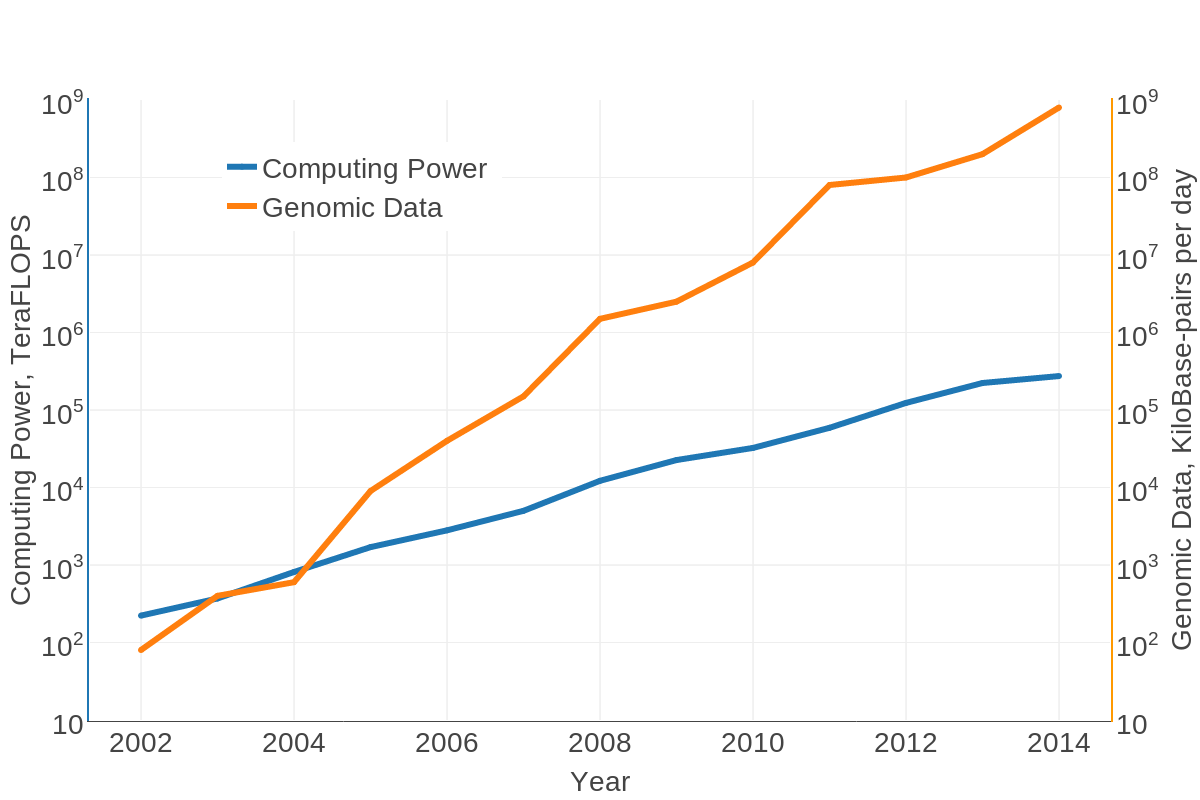
\includegraphics[width=1\textwidth]{assets/computeVsData.png}
        \caption{}
    \end{subfigure}%
    \begin{subfigure}[b]{4in}
        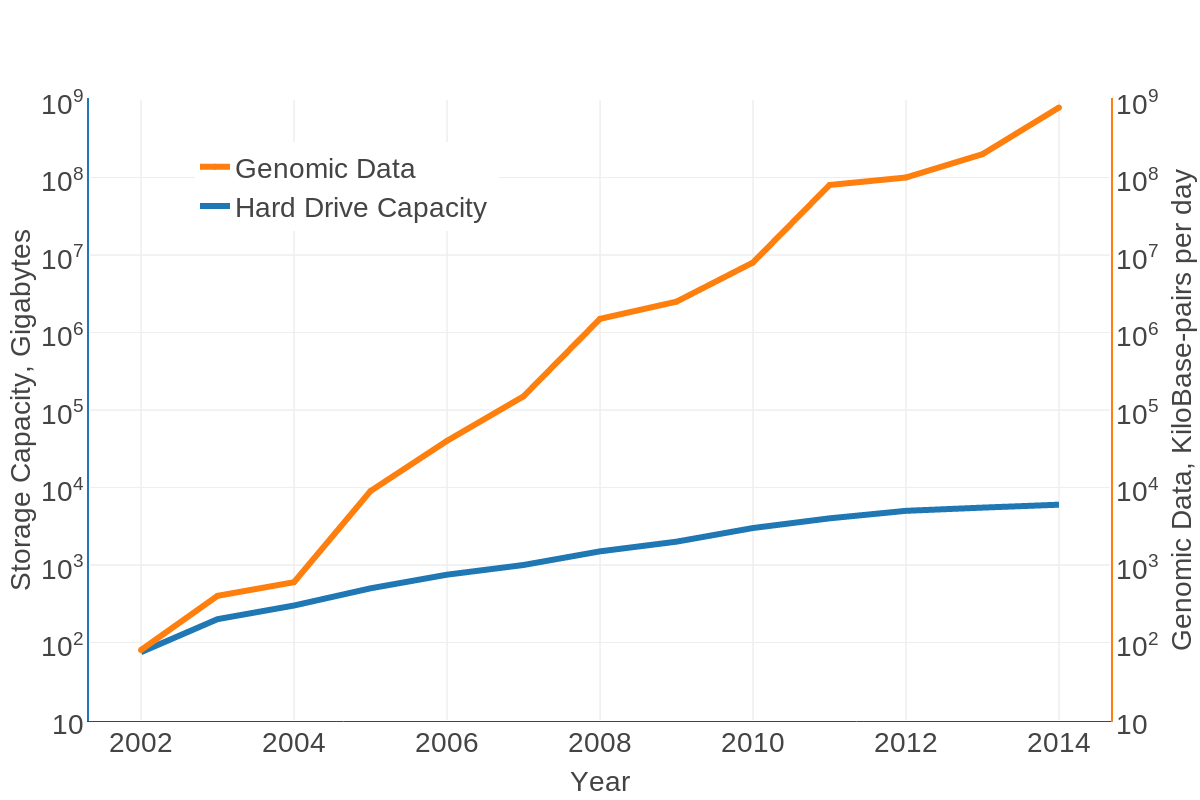
\includegraphics[width=1\textwidth]{assets/storageVsData.png}
        \caption{}
    \end{subfigure}}
    \caption{Genomic data available has grown at a faster exponential rate than computer processing power and disk storage.
    These plots represent, on a log scale, the daily growth in sequence data 
    from GenBank along with (a) the combined computing power (in TeraFLOPs) of 
    the Top 500 Supercomputer list, and (b) the largest commercially-available 
    hard disk drives.}
    \label{fig:expdata}
\end{figure}

\begin{figure}[p]
    \centering
    \vspace{-10em}
    \centerline{
    \begin{subfigure}[b]{3.4in}
        \caption{Cosine distance}
        \label{fig:fragbag_fractal_cosine}
        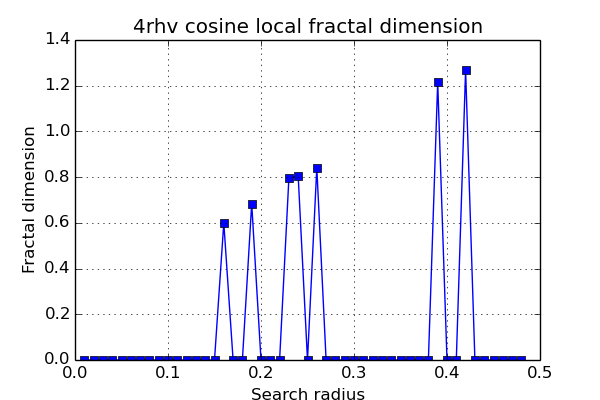
\includegraphics[width=1\textwidth]{assets/4rhv_fractal_cosine.png}
    \end{subfigure}%
    \begin{subfigure}[b]{3.4in}
        \caption{Euclidean distance}
        \label{fig:fragbag_fractal_euclid}
        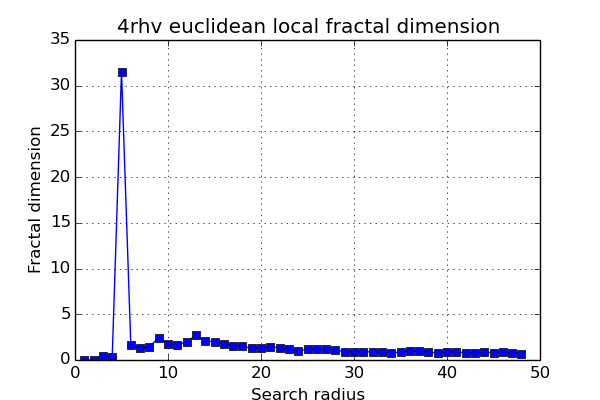
\includegraphics[width=1\textwidth]{assets/4rhv_fractal_euclid.png}
    \end{subfigure}
    }
    \centerline{
    \begin{subfigure}[b]{3.4in}
        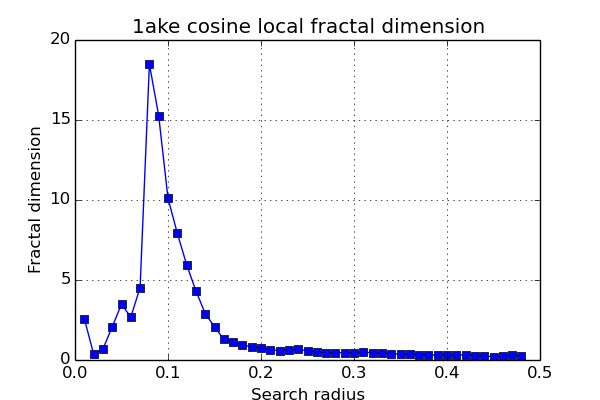
\includegraphics[width=1\textwidth]{assets/1ake_fractal_cosine.png}
        %\caption{}
    \end{subfigure}%
    \begin{subfigure}[b]{3.4in}
        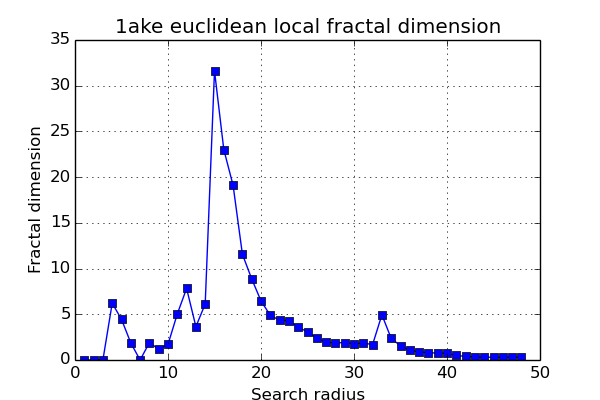
\includegraphics[width=1\textwidth]{assets/1ake_fractal_euclid.png}
        %\caption{}
    \end{subfigure}
    }
    \centerline{
    \begin{subfigure}[b]{3.4in}
        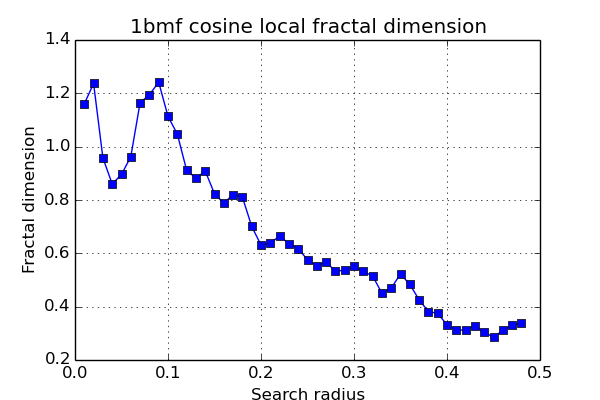
\includegraphics[width=1\textwidth]{assets/1bmf_fractal_cosine.png}
        %\caption{}
    \end{subfigure}%
    \begin{subfigure}[b]{3.4in}
        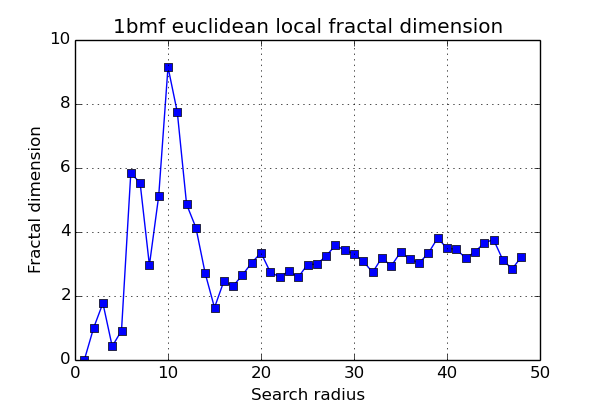
\includegraphics[width=1\textwidth]{assets/1bmf_fractal_euclid.png}
        %\caption{}
    \end{subfigure}
    }
    \centerline{
    \begin{subfigure}[b]{3.4in}
        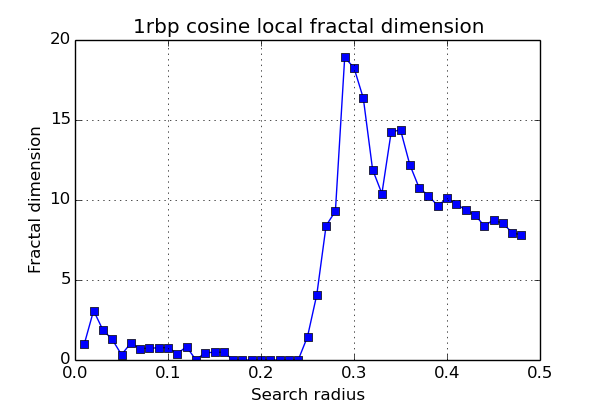
\includegraphics[width=1\textwidth]{assets/1rbp_fractal_cosine.png}
        %\caption{}
    \end{subfigure}%
    \begin{subfigure}[b]{3.4in}
        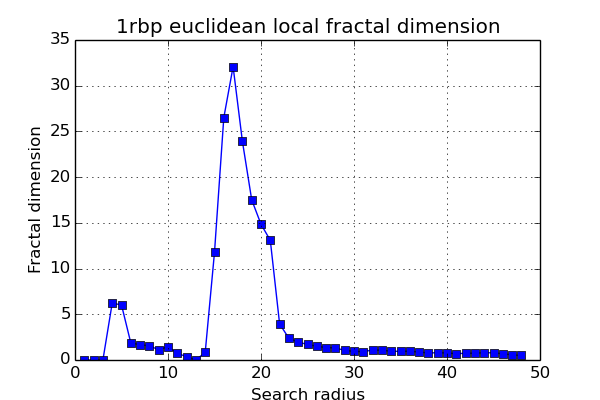
\includegraphics[width=1\textwidth]{assets/1rbp_fractal_euclid.png}
        %\caption{}
    \end{subfigure}
    }
    \caption{Local fractal dimension at different scales for the space of PDB FragBag frequency vectors. Each data point is defined by dimension $d = \frac{\log(n_2/n_1)}{\log(r_2/r_1)}$, where $n_1, n_2$ are the number of similarity search hits within radius respectively $r_1, r_2$, and $r_2 - r_1$ is the increment size of 0.01 for cosine distance and 1 for euclidean distance. In most regimes, local fractal dimension is consistently low, except for a large spike when radius expands to include the central cluster of proteins. esFragBag achieves the most acceleration when both output size is small and we remain in a low fractal dimension regime.}
    \label{fig:fragbag_fractal}
\end{figure}

\section{Supplemental Methods}

\subsection{Theory}
\subsubsection{Time-complexity}
We introduced the definition of the entropy-scaling similarity search data structure in Figure 1.
For ease of analysis, we will work in a high-dimensional metric space and consider the database as a set $D$ of $n$ unique points in that metric space.
Define $B_S(q,r) = \{ p \in S : ||q-p||<r \}$. The similarity search problem is thus to compute $B_D(q,r)$ for a query $q$ and radius $r$.
Note however that the metricity requirement is needed only for a 100\% sensitivity guarantee; other distance functions can be used, but result in some loss in sensitivity.
However, regardless of the distance function chosen, there cannot be a loss of
specificity; false positives will never be introduced because the fine search is just the original search function on a smaller subset of the database.

A set $C$ of $k$ cluster centers are chosen such that no cluster has radius greater than a user-specified parameter $r_c$ and no two cluster centers are within distance $r_c$ of one another.
The data structure then clusters the points in the set by assigning them to their nearest cluster center.
Overloading notation a bit, we will identify each cluster with its center, so $C$ is also the set of clusters.
%We will additionally require that each cluster contain at least $\frac{n}{k \alpha}$ items, for some constant $\alpha \ge 1$ (i.e. that the clusters are balanced).
For a given similarity search query for all items within distance $r$ of a query $q$, this data structure breaks the query into coarse and fine search stages.
The coarse search is over the list of cluster centers, returning $B_C(q,r + r_c)$.
Let \[\displaystyle F = \bigcup_{c \in B_C(q,r+r_c)} c , \] the union of all the returned clusters.
By the Triangle Inequality, $B_D(q,r) \subseteq F$, which combined with $F \subseteq D$ implies that $B_F(q,r) = B_D(q,r)$.
Thus, a fine search over the set $F$ will return all items within radius $r$ of $q$.

Note that we require the metricity requirement only for the Triangle Inequality.
It turns out that many interesting distance functions are not metrics, but still almost satisfy the Triangle Inequality, which is nearly sufficient.
More precisely, if a fraction $\alpha$ of the triples in $S$ do not satisfy the Triangle Inequality, then in expectation, we will have sensitivity $1 - \alpha$.
As shown in the results, empirically, this loss in sensitivity appears to be low and can likely be ameliorated by increasing the coarse search radius.

%We will prove in this section that 
Provided the fractal dimension of the database is low, this data structure allows for similarity search queries in time roughly linear in the metric entropy of the database.
Additionally, without increasing the asymptotic time-complexity, this data structure can also be stored in an \textit{information theoretic} entropy-compressed form.
%Further, as suggested by the last sentence, the metric entropy of the database can be related to the more typical information theoretic notion of entropy (see Supplemental Methods).
%However, to do this, we will first need to build additional mathematical machinery and make precise our notions of `entropy' and `fractal dimension'.

Note that entropy-scaling data structures are distinct from both succinct data structures and compressed data structures.
Succinct data structures are ones that use space close to the information-theoretic limit in the worst case while permitting efficient queries; i.e.
succinct data structures do not depend on the actual entropy of the underlying data set, but have size-dependence on the potential worst-case entropy of the data set \cite{jacobson1988succinct}.
Compressed (and opportunistic) data structures, on the other hand, bound the amount of the space used by the entropy of the data set while permitting efficient queries \cite{grossi2005compressed, ferragina2000opportunistic}.
Entropy-scaling data structures are compressed data structures, but are distinct, as
unlike entropy-scaling data structures, compressed data structures do not measure time-complexity in terms of metric entropy.
Additionally, existing compressed data structures such as the compressed suffix array and the FM-index are designed for the problem of pattern matching \cite{grossi2005compressed, ferragina2000opportunistic}.
While related to similarity search, pattern matching does not admit as general of a notion of distance as the similarity search problem.
While compressed sensing has also been applied to the problem of finding a representative set of genes for a collection of expression samples~\cite{prat2011recovering}, compressed sensing is distinct from entropy-scaling data structures.


\textbf{The primary advance of entropy-scaling data structures is that they bound both space and time as functions of the data set entropy (albeit using two different notions of entropy).}

\subsubsection{Complexity bounds}
We first define the concept of metric entropy and entropy dimension in the usual manner:
\begin{definition}[\cite{tao2008product} Definition 6.1] 
    Let $X$ be a metric space, let $D$ be a subset of $X$, and let $\rho>0$ be a radius.
    \begin{itemize}
        \item The \textit{metric entropy} $N_\rho(D)$ is the fewest number of points $x_1, \ldots, x_n \in D$ such that the balls $B(x_1,\rho), \ldots B(x_n,\rho)$ cover $D$.
    \end{itemize}
\end{definition}
\begin{definition}[\cite{falconer1990fractal}]
    The Hausdorff dimension of a set $D$ is given by 
\[
    \dim_{\text{Hausdorff}}(D) := \lim_{\rho \to 0} \frac{\log N_\rho(D)}{\log 1/\rho}
\]
\end{definition}
Unfortunately, as $D$ is a finite, discrete, set, the given definision always gives $\dim_{\text{Hausdorff}}(D) = 0$.
However, we are only interested in scaling behaviors around large radii, so instead we use:
\begin{definition}
    The fractal dimension $d$ of a set $D$ at a scale $[\rho_1,\rho_2]$ is given by
    \[
        d = \operatorname*{arg\,max}_{d^*} \{ N_\rho(D) \propto \rho^{-d^*} | \rho \in [\rho_1,\rho_2] \}.
    \]
\end{definition}

Recall that $k$ entries are selected as cluster centers for partitioning the database to result in clusters with maximum radius $r_c$.
From the definition above, when setting $\rho = r_c$, it is trivial to verify $ k \le N_{r_c} (D)$.
This upper bound is guaranteed by our requirement that the cluster centers not be within distance $r_c$.

%We will set $r_c = \theta(\frac{1}{k})$.
Given any query $q$, the coarse search over the cluster centers always requires $k$ comparisons.
Additionally, the fine search is over the set $F$, defined to be the union of clusters with centers within distance $r+r_c$ from $q$.
As the time-complexity of similarity search is just the total of the coarse and fine searches, this implies that the total search time is $O(k + |F|)$.

By the triangle inequality, $F \subset B_D(q,r+2r_c)$,
so we can bound $|F| \le |B_D(q,r+2r_c)|$.
Let the fractal dimension $D$ at the scale between $r_c$ and $2r_c + r$ be $d$.
Then in expectation over possible queries $q$,
\[
    \left|B_D(q, r+2r_c)\right| \sim \left|B_D(q,r)\right|\left(\frac{r+2r_c}{r}\right)^d .
\]
Roughly speaking, this scaling argument just says that doubling a search radius only increases the number of hits by a factor of at most $2^d$.
Thus, total search time is 
\[
    O\left(k + \left|B_D(q,r)\right|\left(\frac{r+2r_c}{r}\right)^d \right).
\]
However, note that $k$ is linear in metric entropy and $|B_D(q,r)|$ is the output size, so similarity search can be performed in time linear to metric entropy and a polynomial factor of output size.
Provided that the fractal dimension $d$ is small and $k$ is large, the search time will be dominated by the metric entropy component, which turns out to be the regime of greatest interest for us.
We have thus proven bounds for the time-complexity of similarity search.

\subsubsection{Space-complexity}
Here we relate the space-complexity of our entropy-scaling similarity search data structure to information-theoretic entropy.
Traditionally, information-theoretic entropy is a measure of the uncertainty of a distribution or random variable and is not well-defined for a finite database.
However, the notion of information-theoretic entropy is often used in data compression as a shorthand for the number of bits needed to encode the database, or a measure of the randomness of that database.
We use entropy in the former sense; precisely, we define the entropy of a database as the number of bits needed to encode that database, a standard practice in the field.
Thus, we consider entropy-compressed forms of the original database, such as that obtained by Prediction by Partial Matching (PPM), Lempel-Ziv compression (e.g. Gzip), or a Burrows-Wheeler Transform (as in Bzip2), and use their size as an estimate of the entropy $S_{orig}$ of the database.

For all commonly used compression techniques, decompression time is linear in the size of the uncompressed data.
Obviously, even with linear decompression, decompressing the entire database for each similarity search would squander the entropy-scaling benefits of our
approach.
However, note that the fine search detailed above only needs access to a subset of clusters and furthermore needs full access to that set of clusters.
It is therefore always asymptotically `free' to decompress an entire cluster at once, if any member of that cluster needs to accessed.
Thus, one ready solution is to simply store entropy-compressed forms of each cluster separately.

Compressing each cluster separately preserves runtime bounds, but makes it difficult to compare the compressed clustered database size to the original compressed database size.
This results from the possibility that redundancy across clusters that would originally have been exploited by the compressor can no longer be exploited 
once the database is partitioned.
Intuitively, for any fixed-window or block compressor, grouping together similar items into clusters should increase the performance of the compressor, but it is unclear \textit{a priori} if that balances out the loss of redundancy across clusters.

A somewhat more sophisticated solution is to reorder the entries of the database by cluster, compress the entire database, and then store indexes into the starting offset of each cluster.
For popular tools such as Gzip or Bzip2, this is possible with constant overhead $\kappa$ per index.
Because the entire database is still being compressed, redundancy across clusters can be exploited to reduce compressed size, while still taking advantage of similar items being grouped together.
Thus, in expectation over uniformly-randomly chosen orderings of the database entries (obviously, there is some optimal ordering, but computing that is computationally infeasible), the compressed clustered database size $S_{clust} \le S_{orig}$.
Then, total expected space-complexity of our data structure is $O(\kappa k + S_{orig})$; recall here that $k$ is the number of clusters and is bounded by the metric entropy of the database.
Thus, space complexity is linear in metric entropy plus information-theoretic entropy.

Additionally, given that our distance function measures marginal information-theoretic entropies, we can also give a bound on the total information-theoretic entropy of the database by using metric entropy and the cluster radius.
Let $l$ be the maximum distance of two points in the space.
The na\"ive upper bound on total entropy is then $O(nl)$, where $n$ is the total number of points in the database, because distance and entropy are related.
Recall that we chose $k$ points as cluster centers, where $k$ is bounded by metric entropy, for a maximum cluster radius $r_c$.
Encoding each non-center point $p$ as a function of the nearest cluster center requires $O(n  r_c)$ bits.
Specifying the privileged points again requires $O(kl)$ bits, so together the total information-theoretic entropy is $O(kl + n r_c)$.
In other words, not only is space complexity linear in metric entropy plus information-theoretic entropy, but information-theoretic entropy itself is also bounded by the low-dimensional coarse structure of the database.

\subsubsection{Clustering time}

$O(kn)$ clustering time

$O(k)$ update time (adding a new point).

\subsection{Ammolite}

\subsubsection{Simplification and compression}

Given a molecular graph, any vertex or edge that is not part of a simple cycle or a tree is removed, and any edge that is part
of a tree is removed.
This preserves the node count, but not the topology, of tree-like structures, and preserves simple cycles,
which represent rings in chemical compounds.
For example, as shown in Figure~\ref{fig:ammolite}, both caffeine and adenine would be reduced to a purine-like graph.

After this transformation is applied to each molecule in a database to be compressed, we identify all clusters
of fully-isomorphic transformed molecular graphs.
Isomorphism detection is performed using the VF2~\cite{cordella2001improved} 
algorithm; a simple hash computed from the
number of vertices and edges in each transformed molecular graph is first used 
to filter molecular graphs that cannot possibly be isomorphic.
A representative from each such cluster is stored in SDF format; collectively, these representatives form a 
``coarse'' database.
Along with each representative, we preserve the information necessary to reconstruct each original molecule,
as a pointer to a set of vertices and edges that have been removed or unlabeled.
Clustering is computation- and memory-intensive; clustering the entire 306GiB PubChem database required \textbf{X} days and used \textbf{Y} GiB of RAM.

Ammolite is implemented in Java, and its source code is available on Github.

\subsection{CaBLASTX}

\subsubsection{Alphabet Reduction}

Alphabet reduction---reducing the 20-letter standard amino acid alphabet to a
smaller set, in order to accelerate search or improve homology detection---has
been proposed and implemented several times~\cite{bacardit2007automated, peterson2009reduced}.
In particular, \citet{murphy2000simplified} considered reducing the
amino-acid alphabet to 17, 10, or even 4 letters.
More recently, \citet{zhao2012rapsearch2} and \citet{huson2013poor} applied a reduction to
a 4-letter alphabet, termed a ``pseudoDNA'' alphabet, in sequence alignment.

In this work, we extend the compression approach of 
\citet{daniels2013compressive} using a reversible alphabet reduction.
We use the alphabet reduction of \citet{murphy2000simplified} to map the 
standard amino
acid alphabet (along with the four common ambiguous letters ) onto a 4-letter 
alphabet.
Specifically, we map F, W, and Y into one cluster; C, I, L, M, V, and J into
a second cluster, A, G, P, S, and T into a third cluster, and
D, E, N, Q, K, R, H, B, and Z into a fourth cluster.
By storing the offset of the original letter within each cluster, the original
sequence can be reconstructed, making this a reversible reduction.

\subsubsection{Database Compression}

Given a protein sequence database to be compressed, we proceed as follows:
\begin{enumerate}
        \item First, initialize a table of all possible $k$-mer seeds of
        our 4-letter reduced alphabet, as well as a coarse database of
        reduced-alphabet sequences, initially containing the reduced-alphabet
        version of the first sequence in the input database.
        %
        \item For each $k$-mer of the first sequence, store its position in the
        corresponding entry in the seed table.
        %
        \item For each subsequent sequence $s$ in the input, reduce its 
        alphabet and slide a window of 
        length $k$ along the sequence, skipping single-letter repeats of length
        greater than 10.
        %
        \item
        \begin{enumerate}
        \item Look up these $k$ residues in the seed table.
        For every entry matching to that $k$-mer in the seed table, follow
        it to a corresponding subsequence in the coarse database and attempt
        \textit{extension} (defined below).
        If no subsequences from this window can be extended, move the window
        by $m$ positions, where $m$ defaults to 20.
        \item If a match was found via extension, move the $k$-mer window to
        the first $k$-mer in $s$ after the match, and repeat the extension
        process.
        \end{enumerate}
\end{enumerate}
        
Given a $k$-mer in common between sequence $s$ and a subsequence $s'$ pointed to by the
seed table, first attempt \textit{ungapped} extension:
\begin{enumerate}
        \item Within each window of length $m$ beginning with a $k$-mer match, 
        if there are at least 60\% matches between $s$ and $s'$, then there is 
        an ungapped match.
        \item Continue ungapped matching using $m$-mer windows until no more
        $m$-mers of at least 60\% sequence identity are found.
        \item The result of ungapped extension is that there is an alignment 
        between $s$ and $s'$ where the only differences are substitutions,
        at least 60\% of the positions contain exact matches.
\end{enumerate}
        
When ungapped extension terminates, attempt \textit{gapped} extension.
From the end of the aligned regions thus far, align 25-mer windows of both
$s$ and $s'$ using the Needleman-Wunsch~\cite{needleman1970general} algorithm 
using an identity matrix.
Note that the original caBLASTP~\cite{daniels2013compressive} used BLOSUM62 as 
it was
operating in amino acid space; as we are now operating in a reduced-alphabet
space, an identity matrix is appropriate, just as it is for nucleotide space.
After gapped extension on a window length of 25, attempt ungapped extension
again.

If neither gapped nor ungapped extension can continue, end the extension phase.
If the resulting alignment has less than 70\% sequence identity (in the 
reduced-alphabet space), or is shorter than 40 residues, discard it, and 
attempt extension on the next entry in the seed table for the original $k$-mer,
continuing on to the next $k$-mer if there are no more entries.

If the resulting alignment does have at least 70\% sequence identity in the
reduced-alphabet space, and is at least 40 residues long, then create a link
from the entry for $s'$ in the coarse database to the subsequence of $s$
corresponding to the alignment.
If there are unaligned ends of $s$ shorter than 30 residues, append them to the
match.
Longer unaligned ends that did not match any subsequences reachable from the
seed table are added into the coarse database themselves, following the same
$k$-mer indexing procedure as the first sequence.

Finally, in order to be able to recover the original sequence with its original
amino acid identities, a \textit{difference script} is associated with each
link.
This difference script is a representation of the insertions, deletions, and
substitutions resulting from the Needleman-Wunsch alignment, along with the
offset in each reduced-alphabet cluster needed to recover the original alphabet.
Thus, for example, a valine (V) is in the cluster containing C, I, L, M, V, and 
J.
Since it is the 4th entry in that 5-entry cluster, we can represent it with
the offset 4.
Since the largest cluster contains 9 elements, only four bits are needed to
store one entry in the difference script.
More balanced clusters would have allowed 3-bit storage, but at the expense of
clusters that less faithfully represented the BLOSUM62 matrix and the
physicochemical properties of the constituent amino acids.

Because of the seed table, compression is memory-intensive and CPU-intensive.
Compressing the September, 2014 NCBI NR database required approximately 120 hours on a 12-core Xeon with 88GB RAM.



\subsubsection{Query Clustering}

Metagenomic reads are themselves nucleotide sequences, so no alphabet reduction
is performed on them directly.
Instead, metagenomic reads are compressed using the same approach as the
protein database, without the alphabet reduction step and with a number of
different parameters.
The difference scripts for metagenomic reads do not rely on the cluster offsets,
but simply store the substituted nucleotides.

Furthermore, unlike protein databases, where most typical sequences range in 
length from 100 to over 1000 amino acids, next-generation sequencing reads are 
typically short and usually of fixed length, which is known in advance.
Thus, the minimum alignment length required for a match, and the maximum
length unaligned fragment to append to a match, require different values based
on the read length.

An additional complication is that insertions and deletions from one read to
another will change the reading frame, potentially resulting in 
different amino acid sequences.
For this reason, query clustering requires long, \emph{ungapped} windows of high
sequence identity.
Specifically, for 202-nucleotide reads, for two sequences to cluster together,
we require a 150-nucleotide ungapped region of at least 80\% sequence identity.

In the future, we may consider first translating the reads, and performing
clustering in the amino acid space (after alphabet reduction).
This would have the advantage of allowing reads with insertions or deletions
to cluster together, without causing reading-frame mismatches.
However, gapped alignment is much slower than ungapped alignment,
so the resulting cost of query clustering might negate speed gains.

We note that unlike the compression of the database, which can be amortized 
over future queries, the time spent clustering and compressing the queries 
cannot be amortized.
Thus, we would not refer to the query clustering as entropy-scaling, but it
still provides a constant speed-up.
For this reason, we include the time spent clustering and compressing queries in the search time for caBLASTX.


\subsubsection{Search}

Given a compressed protein database and a compressed query read set, search
comprises two phases.
The first, \emph{coarse search}, considers only the coarse sequences---the
representatives---resulting from compression of the protein database and the
query set.
Just as with standard BLASTX, each coarse nucleotide read is transformed into 
each of the six possible amino acid sequences that could result from it (three 
reading frames for both the sequence and its reverse complement).
Then, each of these amino acid sequences is then reduced back to a four-letter
alphabet using the same mapping as for protein database compression.
For convenience, the four-letter alphabet is represented using the standard
nucleotide bases, though this has no particular biological significance.
This is done so that the coarse search can rely on BLASTN (nucleotide BLAST) to
search these sequences against the compressed protein database.

For each coarse query representative (identified using a a coarse E-value of 
1000, along with the BLASTN arguments \texttt{-task blastn-short -penalty -1}), 
the set of coarse hits is used to
reconstruct all corresponding sequences from the original database by following
links to original sequence matches and applying their difference scripts.
The resulting \emph{candidates} are thus original sequences from the protein
database, in their original amino acid alphabet.
The query representative is also used to reconstruct all corresponding sequences
from the original read set.
Thus, for each coarse query representative, there is now a subset of the
metagenomic read set (the reads represented by that coarse query) and also a
subset of the protein database (the candidates).

The second phase, \emph{fine search}, uses standard BLASTX to translate each
of these reads associated with a coarse query representative and search for
hits only in the subset of the database comprising the candidates.
This fine search phase relies on a user-specified E-value threshold (defaulting
to BLASTX's default of 10) to filter hits.
To ensure that E-value calculation is correct, BLASTX uses a corrected database
size which is the size of the original, uncompressed protein database.

\subsubsection{Benchmarking}

Although our primary result is the direct acceleration of BLASTX using our
entropy-scaling data structures, we also compared caBLASTX to 
RapSearch2~\cite{zhao2012rapsearch2} version 2.22 and the November 29, 2014 
version of Diamond~\cite{buchfink2014fast}.
All tests were performed on a 12-core Intel Xeon X5690 running at 3.47GHz with
88GB RAM and hyperthreading; 24 threads were allowed for all programs.
Diamond was run with the \texttt{--sensitive} option.
In all cases, an E-value threshold of \texttt{1e-7} was used.

For the raw-read dataset, we filtered out reads starting or ending with 10 or 
more no-calls ('N').

CaBLASTX is implemented in Go, and its source code is available on Github.

\subsection{esFragBag}
We took the existing FragBag method as a black box and by design did not do anything clever in esFragBag except apply the entropy-scaling similarity search data structure.
Additionally, we removed the sorting-by-distance feature of Andrew Gallant's 
FragBag search function, which does not improve the all-matching results we 
were interested in here---it lowers $k$-nearest neighbor search memory 
requirements while dominating the running time of $\rho$-nearest neighbor, the 
problem at hand.
This was done for both the FragBag and the esFragBag benchmarks, to ensure comparability.
All code was written in Go, and is available on Github.

The entire 2014 Oct 31 version of the Protein Data Bank was downloaded and the 
database was composed of fragment frequency vectors generated from all of the 
relevant PDB files using the 400-11.json fragment list \cite{budowski2010fragbag}.
For this paper, we implemented the benchmarking in Go, and have provided the 
source code for the benchmarking routine on Github.
This allowed us to benchmark just the search time, excluding the time to load the database from disk.
Note that the prototype implementation of esFragBag available only supports the 
all $\rho$-nearest neighbor search query found in FragBag.

\bibliographystyle{model5-names-noitalic}
%\bibliographystyle{plain}
\bibliography{main}


\end{document}
